\documentclass[11pt,a4paper]{article}

\usepackage[utf8]{inputenc}
\usepackage[english]{babel}
\usepackage[T1]{fontenc}
\usepackage{graphicx}
\usepackage{hyperref}
\usepackage{caption}
\usepackage{subcaption}

\usepackage{amsmath,amssymb,amsfonts}

\title{Principles of Computer System Design\\Assignment 3}
\author{Kristoffer Søholm\\Sebastian Paaske Tørholm}

\begin{document}
\maketitle

\section{Exercises}
\subsection{Question 1: Recovery Concepts}
\subsubsection{Subquestion 1}
It is not necessary to implement neither redo nor undo. Redo is necessary if
there is not guarantee that the data will be written to persistent storage,
however with force this guarantee is in place. Similarly, undo is needed if we
can read uncommitted data, as there is a possibility that the data will not end
up being committed, so the action involving the data will need to be undone.
This cannot happen, since we don't allow stealing of locked data.

\subsubsection{Subquestion 2}
Nonvolatile storage is storage that is preserved across system failures or
restarts, but which has no other guarantees and might be lost to disk failure,
corruption or similar. In contrast, stable storage gives the hypothetical
guarantee that the data is never lost. This is most often approximated through
data replication, for example tape backups, external disks, off-site backups,
crystals\footnote{\url{http://physicsworld.com/cws/article/news/2013/jul/17/5d-superman-memory-crystal-heralds-unlimited-lifetime-data-storage}} etc. 
Stable storage is intended to survive through all failures, most commonly disk
failure, corruption, natural disasters such as fires or floods, and human
error.

\subsubsection{Subquestion 3}
When employing Write-Ahead Logging, we have two situations when log records
need to be forced to disk.

When updating data, we need to write the log record for the update to disk
before the data itself reaches the disk. If we don't do this, we risk the
system going down with the data written, but no log entry for the given
change. This is a problem if we need to roll back the transaction writing
the data, since the original data then is gone. By writing the log record,
we ensure that we have the possibility of doing this undo even if the system
crashes.

When committing a transaction, all log records for that transaction need to be
written to disk before the commit can take place. A situation where not upholding
this is a problem is as follows:

\begin{itemize}
    \item T1 updates X, log record for this update isn't written to disk.
    \item T1 commits.
    \item T2 starts a transaction updating X, writes log entry to disk.
    \item System crashes.
\end{itemize}

If we now need to recover, we erroneously omit the changes done to X by T1,
which T2 was meant to use.

By forcing the log of a transaction before committing, we ensure that any
transaction depending on it cannot obtain a lock on the data before we know
that the changes are stored persistently, and thus will not be lost.

\subsection{Question 2: ARIES}
We start by running the analysis phase, obtaining \autoref{xact-table} and \autoref{dirty}.

\begin{figure}[h!]
    \centering
\begin{tabular}{|c|c|c|}
    \hline
    Xid & LastLSN & Status \\
    \hline
    T1  & 4       & Running \\
    T2  & 9       & Running \\
    \hline
\end{tabular}
\caption{Transaction table after analysis phase}
\label{xact-table}
\end{figure}

\begin{figure}[h!]
    \centering
\begin{tabular}{|c|c|c|}
    \hline
    PageId & recLSN \\
    \hline
    P1     & 4 \\
    P2     & 3 \\
    P3     & 6 \\
    P5     & 5 \\
    \hline
\end{tabular}
\caption{Dirty page table after analysis phase}
\label{dirty}
\end{figure}


As we can see from \autoref{xact-table}, the loser transactions are
$\{T1,T2\}$, and the winner transactions are $\{T3\}$ since it does not appear.

The redo phase starts on $LSN = 3$, since that is the lowest $LSN$ in the dirty
page table. During the redo-phase, the set of log records that may cause pages
to be rewritten is $\{3,4,5,6,8,9\}$. The reason why they might not be
rewritten is that they are already flushed to the disk, which is the case if
$pageLSN \geq LSN$ for the given log record.

After the undo phase, the log is as follows:

\begin{verbatim}
LOG

LSN   LAST_LSN    TRAN_ID    TYPE               PAGE_ID
---   --------    -------    ----               -------
1     -           -          begin CKPT         -
2     -           -          end CKPT           -
3     NULL        T1         update             P2
4     3           T1         update             P1
5     NULL        T2         update             P5
6     NULL        T3         update             P3
7     6           T3         commit             -
8     5           T2         update             P5
9     8           T2         update             P3
10    6           T3         end                -
11    CLR undo T2, LSN=9, nextCLR=8             P3
12    CLR undo T2, LSN=8, nextCLR=5             P5
13    CLR undo T2, LSN=5, nextCLR=NULL, T2 end  P5
14    CLR undo T2, LSN=4, nextCLR=3             P1
15    CLR undo T2, LSN=3, nextCLR=NULL, T1 end  P2
\end{verbatim}

The toUndo set is empty after undoing $LSN = 3$, so the undo phase ends. From
the CLR's in the final log, we can see that the log records $\{3,4,5,8,9\}$
were undone.

\section{Implementation}


\section*{Experiment}
\subsection*{Dataset}
The dataset is generated by the {\it BookSetGenerator} class, which generates
books with randomized ISBNs, titles, and authors. The price of the books is set
to be in the range $1 \leq \mathtt{price} \leq 301$. Thus, the dataset should
capture all types of books, and although they might not appear in normal ratios
we se no reason why this should be a limiting factor for the validity of the
experiment.

The amount of books is initially set to $100$, each with $200-400$ copies.
The amount of books is another very interesting factor to vary, but for this
experiment it had to be fixed. The number is a bit arbitrary and probably a
good deal on the low side for a growing company, but we also needed a number
which is manageable for our test machine. The amount of copies are chosen so
that a high amount of interactions are successful, as our data analysis depends
on the assumption that $\mathtt{throughput} \approx \mathtt{goodput}$.

\subsection*{Hardware}
In our experiment, we ran the test implemented in the \texttt{main} method of
\texttt{CertainWorkload} twice - once using the local methods, and once using
the RPC interface (but running on the same machine). The tests were run in the
following environment:

\begin{verbatim}
Test setup
----------
CPU: Intel Core i7-3612QM CPU @ 2.10GHz
Memory: 12 GB DDR3 1600MHz RAM
OS: Ubuntu 13.10, kernel 3.11.0-14-generic (x86-64) 
Java: java version 1.7.0_25, OpenJDK Runtime Environment (IcedTea 2.3.12)
\end{verbatim}
\subsection{}

\subsection*{Results}

The experiments were run with up to 14 parallel consumers, at which point the
system was noticably constained by the load.

The resulting data has been plotted and can be seen in \autoref{throughput}
and \autoref{latency}. We have chosen to plot the local and proxied benchmarks
independently, since the scales are so widely different on the two datasets
that plotting them together makes the data inlegible.

\begin{figure}[h!]
    \centering
    \begin{subfigure}[b]{.4\textwidth}
        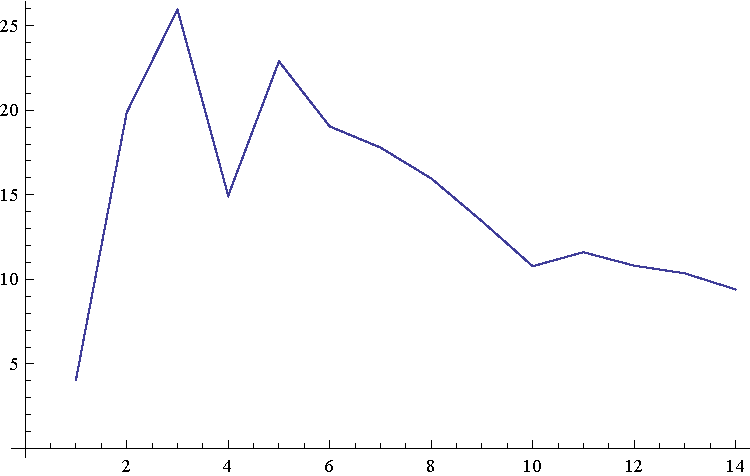
\includegraphics[width=\textwidth]{../analysis/throughput-local-kris.pdf}
        \caption{Local test}
    \end{subfigure}
    \,
    \begin{subfigure}[b]{.4\textwidth}
        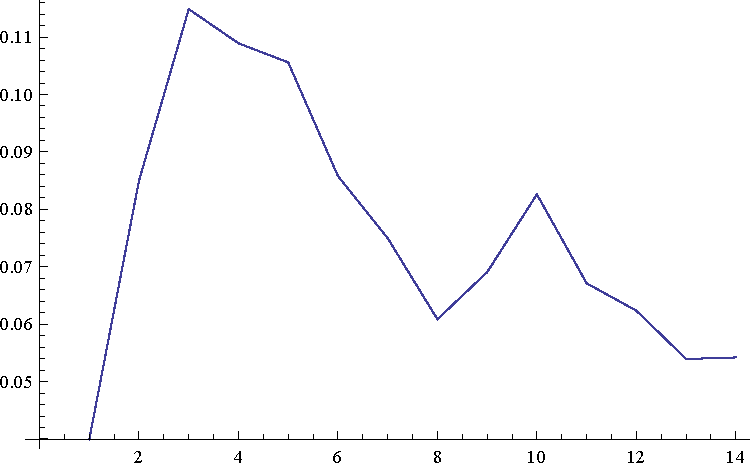
\includegraphics[width=\textwidth]{../analysis/throughput-remote-kris.pdf}
        \caption{Proxied test}
    \end{subfigure}
    \caption{Throughput in operations/ms plotted against number of parallel consumers}
    \label{throughput}
\end{figure}

\begin{figure}[h!]
    \centering
    \begin{subfigure}[b]{.4\textwidth}
        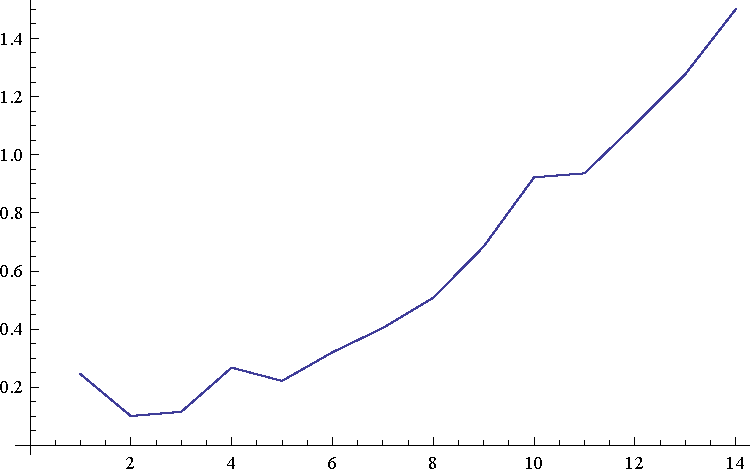
\includegraphics[width=\textwidth]{../analysis/latency-local-kris.pdf}
        \caption{Local test}
    \end{subfigure}
    \,
    \begin{subfigure}[b]{.4\textwidth}
        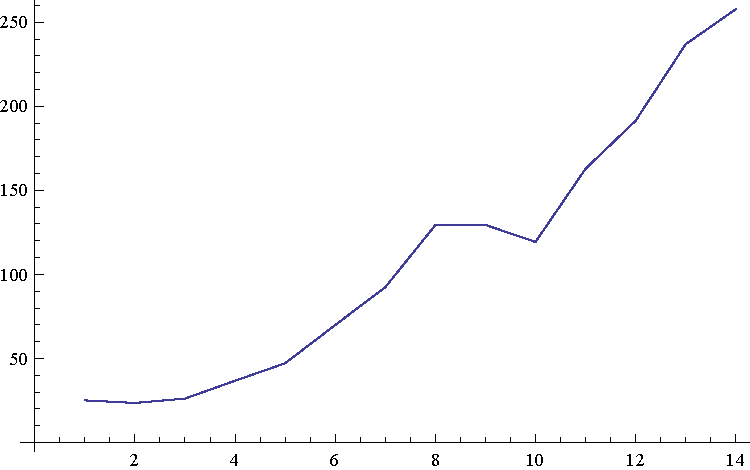
\includegraphics[width=\textwidth]{../analysis/latency-remote-kris.pdf}
        \caption{Proxied test}
    \end{subfigure}
    \caption{Average latency in ms plotted against number of parallel consumers}
    \label{latency}
\end{figure}

For throughput we expect to see a high throughput for a low number of parallel
consumers, with the throughput decreasing as the number of consumers increase.
The low concurrency means that it shouldn't take more than a few threads to
max out the capacity of the service. Since the amount of work to be done in
total grows with the number of threads, this should lead to a decrease in
throughput once the capacity is reached.

In \autoref{throughput} we see that the maximum capacity is reached around
$2-3$ simulataneous threads, decreasing thereafter. There does appear to be a
spike around $10$ simultaneous threads which we cannot explain.

For latency we expect the latency to be low for a low number of
consumers, increasing with the number of consumers due to having to wait for
the resource to be free.

The graphs in \autoref{latency} confirm this theory, showing a significant
increase in latency as the number of threads go up.

\section{Discussion of Implementation}

\end{document}

